\documentclass[table, 12pt]{article}
\usepackage{graphicx}
\usepackage[T1]{fontenc}
\usepackage{tocloft}
\usepackage{todonotes}
\usepackage{caption}
\usepackage{hyperref}
\usepackage{booktabs}
\usepackage{listings}
\usepackage{pdfpages}
\usepackage{pdflscape}
\usepackage{scrhack}
\usepackage{xcolor}
\usepackage{float}
\usepackage{longtable}
\usepackage{enumitem}
\usepackage{tasks}

\begin{document}
\begin{titlepage}
    \centering
    {\scshape\large AY 2020/2021 \par}
    \vfill
    
\includegraphics[width=100pt]{assets/logo-polimi-new}\par\vspace{1cm}
    {\scshape\LARGE Politecnico di Milano \par}
    \vspace{1.5cm}
    {\huge\bfseries RASD\@: Requirement Analysis
        and Specification Document \par}
    \vspace{2cm}
    {\Large {Alice Piemonti\quad Luca Pirovano\quad Nicolò Sonnino}\par}
    \vfill
    {\large Professor\par
        Matteo \textsc{Rossi}}
    \vfill
    {\large \today \par}
\end{titlepage}
\hypersetup{%
    pdfborder = {0 0 0}
}
\thispagestyle{plain}
\pagenumbering{gobble}
\mbox{}
\newpage
\pagenumbering{roman}
\tableofcontents
\newpage
\pagenumbering{arabic}
\section{Introduction}
CLup (Customers Line-up) is an easy-to-use application which intent is to help grocery shopping to face the big challenges that arise during this tough period.

In fact, due to the recent worldwide spread of SARS-CoV-2 (COVID-19), many countries are imposing lockdowns and strict regulations about social distancing such as: the closure of restaurants in the evening, limitations on public transports, curfews, etc.\\

In particular, supermarkets are imposed to restrict accesses to their stores, in order to avoid having too much people inside them, which stands at the basis of social distancing. Furthermore, the staggered access needed by stores lead to the same problem in the outside, such as long queues and crowds.

Grocery stores need an application which main intent is to manage in an efficient way customers arrival on the outside of the supermarket, and to count the access of people inside them. The advantage is to regulate the influx of people near the stores, according to the applicable strict rules, and to avoid long hours of waiting, saving people from line up.

\subsection{Purpose}
The aim of the product is to avoid gatherings outside and inside grocery stores,  improving the safety of the customers.

This is achieved through monitoring accesses to the buildings, managing time slots for visits and optimizing people flows inside the stores.\\

The application should provide two types of accesses for customers (as normal users) and stores' attendants (as special users).

Customers will have the possibility to line up in a virtual queue, so that they can wait from a close and safe building until their number is called. In a reasonable time, the application will inform the user when his number is about to be called, so that he can reach the store in the right time.\\

In addition, users can book a visit to the supermarket for a different time or day. Hence, the customer indicates the slot preferred and, if it is available, the application register the reservation; otherwise a list of alternatives are displayed, such as the possibility to book in a different slot, or to chose different stores available for that time/day.\\

The application can also register in advance the duration of the visit of a customer, and a list of categories that the customer intends to buy, so that the system can suggest the best slot and plan in a finer way the visits, in order to guarantee a correct distance through the aisles inside the store. In fact, the application will be able to balance the presence of people in all the areas of the supermarket, as well as the flows of visitors throughout the day.

Customers will be able to activate an additional functionality: the application will send a notification of available slots in a certain day/time range. Hence, the user will be facilitated in the search of an available slot, and this will guarantee that the user won't spend too much time managing the reservations.\\

Attendants will have the possibility to scan a QR code (generated by the user's application) at the entrance of the store with a specific functionality offered by the application itself; this helps the attendants to verify the correctness of customers' arrivals and, in the meanwhile, monitor the number of entrances.

In addition, attendants will have access to a proper area of the application that permits to behave as a proxy and hand out tickets on spot, in order to guarantee the access to those people who doesn't have access to the application (elderly people, people who don't have a smartphone or an Internet access).\\

The application will be operable freely, widely available and very intuitive, because the range of users (i.e. people who need to go to the grocery store) extends to the entire population.

The user base is expected to be both people with an Internet access and ones without it, from young people to elderly, thanks to the possibility of attendants to act as a proxy.

\subsection{Scope}
The product shall be called CLup and will let users to plan their shopping session in two different ways:
\begin{itemize}
    \item {\textbf{ASAP}: the user will claim the first available ticket and receive an estimated queue time.}
    \item {\textbf{Reservation}: the user will choose a day/time slot from a list of available ones, in order to book his visit to the structure.}
\end{itemize}

Every customer can choose one of these modalities \textbf{remotely} via an official app or through a web browser, or \textbf{in presence} by asking to a staff member, who will act as an intermediate between the customer and the system.

When a customer makes a reservation, the system allows him to choose the duration of his visit and insert a list of possible purchases, in order to optimize his stay.\\

In addition to that, the user can change both the slot and the store relying on system's suggestions: the application will display the best recommendation in order to balance the number of people inside a store throughout the day, merging in the same time slots those people who will purchase different product, in order to guarantee a good distancing through the aisles as well. The user can also enable periodically notifications of available slots in a day/time range: this will allow the application to notify the user when a desirable slot (according to day/time preferences) is available.


\todo{aggiungere introduzione e nome sottosezione}
\begin{center}
    \begin{table}
        \rowcolors{3}{blue!15}{white}
        \begin{tabular}{|c|c|c|}
            \hline
            \rowcolor{blue!50}
            Phenomenon                                 & Who controls it? & Is shared? \\
            \hline
            The formation of queues                    & W                & N          \\
            Social distancing                          & W                & N          \\
            User registration                          & M                & Y          \\
            User login                                 & W                & Y          \\
            Check username and password                & M                & N          \\
            User retrieves a new number                & W                & Y          \\
            Generate a unique number                   & M                & N          \\
            Visualize queue number                     & W                & Y          \\
            Check time-out                             & M                & N          \\
            Notify number is going to be called        & M                & Y          \\
            Generate a QR code                         & M                & N          \\
            Visualize QR code                          & M                & Y          \\
            Attendant scans QR code                    & W                & Y          \\
            Check QR code validity                     & M                & N          \\
            Customer retrieves a number on spot        & W                & Y          \\
            User selects day/time of slot              & W                & Y          \\
            Check availability of slot                 & M                & N          \\
            User adds visit duration                   & W                & Y          \\
            Check visit duration validity              & M                & N          \\
            User indicates list of items               & W                & Y          \\
            Confirm slot has been reserved             & M                & Y          \\
            Cross data                                 & M                & N          \\
            Make recommendation of alternative slots   & M                & N          \\
            Visualize suggestions of alternative slots & M                & Y          \\
            Check customers balance                    & M                & N          \\
            Accept receipt of notifications            & W                & Y          \\
            Search periodically for available slots    & M                & N          \\
            Notify for available slots                 & M                & Y          \\

            \hline
        \end{tabular}
        \caption{phenomena table}
    \end{table}
\end{center}
\newpage
\subsection{Goals}
\label{goals}
The main objectives of our system are the following:
\begin{itemize}
    \item {\textbf{G1: Allow users to retrieve a unique queue number}\\This is the main feature of the application, through which customers are invited not staying outside the structure. Through an appropriate estimation of each customer's permanence time, the user receives an estimated queue time after which he can go to the store. The number is guaranteed to be unique.}
    \item {\textbf{G2: Allow users to generate a QR Code}\\The QR Code is needed in order to let store attendants to monitor entrances, scanning the customer's code upon entering.}
    \item {\textbf{G3: Allow shops to offer this service}\\This goal can be split into the following:
          \begin{itemize}
              \item {\textbf{Allow shops to offer the remote queue function}\\Each shop can register to the service and let customers to Line-Up from home. The application will track the state of the queue.}
              \item {\textbf{Allow shops to generate tickets on the spot}\\If someone does not have access to the required technology, they can still take advantage of the system by getting their queue number directly at the store, where an attendant will act as an intermediate.}
          \end{itemize}
          }
    \item {\textbf{G4: Allow users to "book a visit"}\\Users can book a slot providing the expected duration of the visit. Moreover, users can provide a list which describes the categories of products they intend to buy. Thank to this, visits are optimized and those customers who belong to the same slot, are supposed to buy different types of product, so that they stay in different areas of the store.}
    \item {\textbf{G5: Let the system to infer a visit duration}\\For long term users, the system provides an estimation of visit duration, relying on their previous shopping sessions data.}
    \item {\textbf{G6: Allow users to receive a suggestion of alternative slots}\\During the reservation procedure users will receive a list of alternatives. This help to balance out the number of people in the store during the day. The suggestions could be both on the same shop chain and on different chains.}
    \item {\textbf{G7: Allow users to receive notifications on available slots}\\Users could enable notifications in order to receive periodic announcements of available slots in a preferred day/time range.}
\end{itemize}
\subsection{Definitions, Acronyms, Abbreviations}
\subsubsection{Definitions}
\begin{itemize}
    \item \textbf{Customers:} the people whom this service is directed. They can belong to any age and sex. Their main purpose is to request a ticket to schedule their line up at the shop.
    \item \textbf{User:} it is a customer who uses the application.\label{User}
    \item \textbf{Store:} it is the provider of the goods that customers want to buy. It is obliged to limit the number of people entering in its building through a line up method, in order to respect the local laws for COVID-19 pandemic.
    \item \textbf{Attendant:} it is a store's employee. Its aim is both to manage entrances and to help customers. For this reasons attendants can scan QR codes from customers' application and also release tickets on spot acting as intermediate for customers.
    \item \textbf{Store Administrator:} it is the profile of the store's page creator. It can manage opening hours, available slots, people per slot, etc.
    \item \textbf{Queue number:} it is the ID assigned to each user. It's composed of alphanumerical elements, and it's needed to access the desired shop. It can be retrieved online or on the spot.
    \item \textbf{Visit:} it refers to the customers entering the shop, and also to their staying time. It is associated to both a certain store and a day/time range.
    \item \textbf{Slot:} it is a day/time range. It can be reserved by a limit number of users in order to guarantee a maximum number of people who are inside a store in every time of the day.
    \item \textbf{QR Code:} it's a graphic representation of a string, which can be easily read through barcode readers. It contains the visual representation of the queue number, in order to let attendants make a customer "check-in".\label{QR}
    \item \textbf{Notification:} it's an alert that a certain event occurred. This alert can be a "Push Notification" on the smartphone, an SMS, an email and so on.
    \item \textbf{Push notification:} it's an automated message sent by an application to a user when the application is not running.
    \item \textbf{Actor:} user, attendant or store administrator.
    \item \textbf{Man in the Middle:} it is a cyberattack where the attacker secretly relays and possibly alters the communications between two parties who believe that they are directly communicating with each other.
\end{itemize}
\subsubsection{Acronyms}
\begin{itemize}
    \item {\textbf{ASAP:} As Soon As Possible. It refers to the possibility of getting an appointment on the first available slot.}
    \item {\textbf{S2B:} Software to Be, it is the one designed in this document and not yet implemented.}
    \item {\textbf{API:} Application Programming Interface, it indicates on demand procedure which supply a specific task.}
    \item \textbf{DBMS:} Data Base Management System, it is an interface between the end user and the database, simultaneously managing the data, the database engine, and the database schema in order to facilitate the organization and manipulation of data.
    \item {\textbf{UML:} Universal Modelling Language, it is a way of designing application based on its graphic class representation.}
    \item \textbf{BPMN:} Business Process Model and Notation, it is a graphical representation for specifying business processes in a business process model.
    \item \textbf{SSL:} Secure Socket Layer, it is a secure protocol developed for sending information securely over the Internet.
\end{itemize}
\subsubsection{Abbreviations}
\begin{itemize}
    \item {\textbf{ID:} identifier. It's a generally unique sequence of numbers or letters in order to unambiguously identify an entity.}
    \item {\textbf{Gn:} goal number n}
    \item \textbf{Dn:} domain assumption number n
\end{itemize}
\subsection{Revision History}
\subsection{Reference Documents}
\begin{itemize}
    \item {Specification document: "R\&DD Assignment A.Y. 2020-2021"}
    \item {Alloy official documentation: \href{https://alloytools.org/documentation.html}{https://alloytools.org/documentation.html}}
    \item {Paper: "Jackson and Zave: the world and the machine"}
    \item {UML official specification \href{https://www.omg.org/spec/UML/}{https://www.omg.org/spec/UML/}}
\end{itemize}
\subsection{Document Structure}
\begin{itemize}
    \item {\textbf{Section 1: Introduction}\\This section offers a brief description of the problem and required functionalities. \\It also contains the list of definitions, acronyms and abbreviations that could be found in this document. \\Finally, there are changelog of the document, containing the revisions list and their content, and document structure, which describes the main purposes of the sections of this document.}
    \item {\textbf{Section 2: Overall Description}\\This section offers a summary description about the overall organization of the system, the Hardware and Software constraints and the interfaces needed to get it work.\\It also contains a description of all the features offered by the application, and of the actors who use it.}
    \item {\textbf{Section 3: Specific Requirements}\\This section contains several visual mockups in order to explain the interfaces listed in Section 2. It also contains a description of functional requirement through some scenarios, use cases and diagrams.}
    \item {\textbf{Section 4: Formal Analysis through Alloy}}
\end{itemize}
\newpage
\section{Overall Description}
\subsection{Perspective}
CLup is a complete system that offers the functionalities described in the specific \textit{Product Functions (\ref{product_functions})} section.

It does not lean on a previously existent system and does not offer integrations with other existing systems.

CLup provides all the module that are necessary for its execution. However, it must exploit external interfaces to accomplish its requirements.

We can see a brief report of the information stored by the application through the class diagram of figure \ref{class_diagram}.

\begin{figure}
    \begin{center}
        \hspace*{-1.5in}
        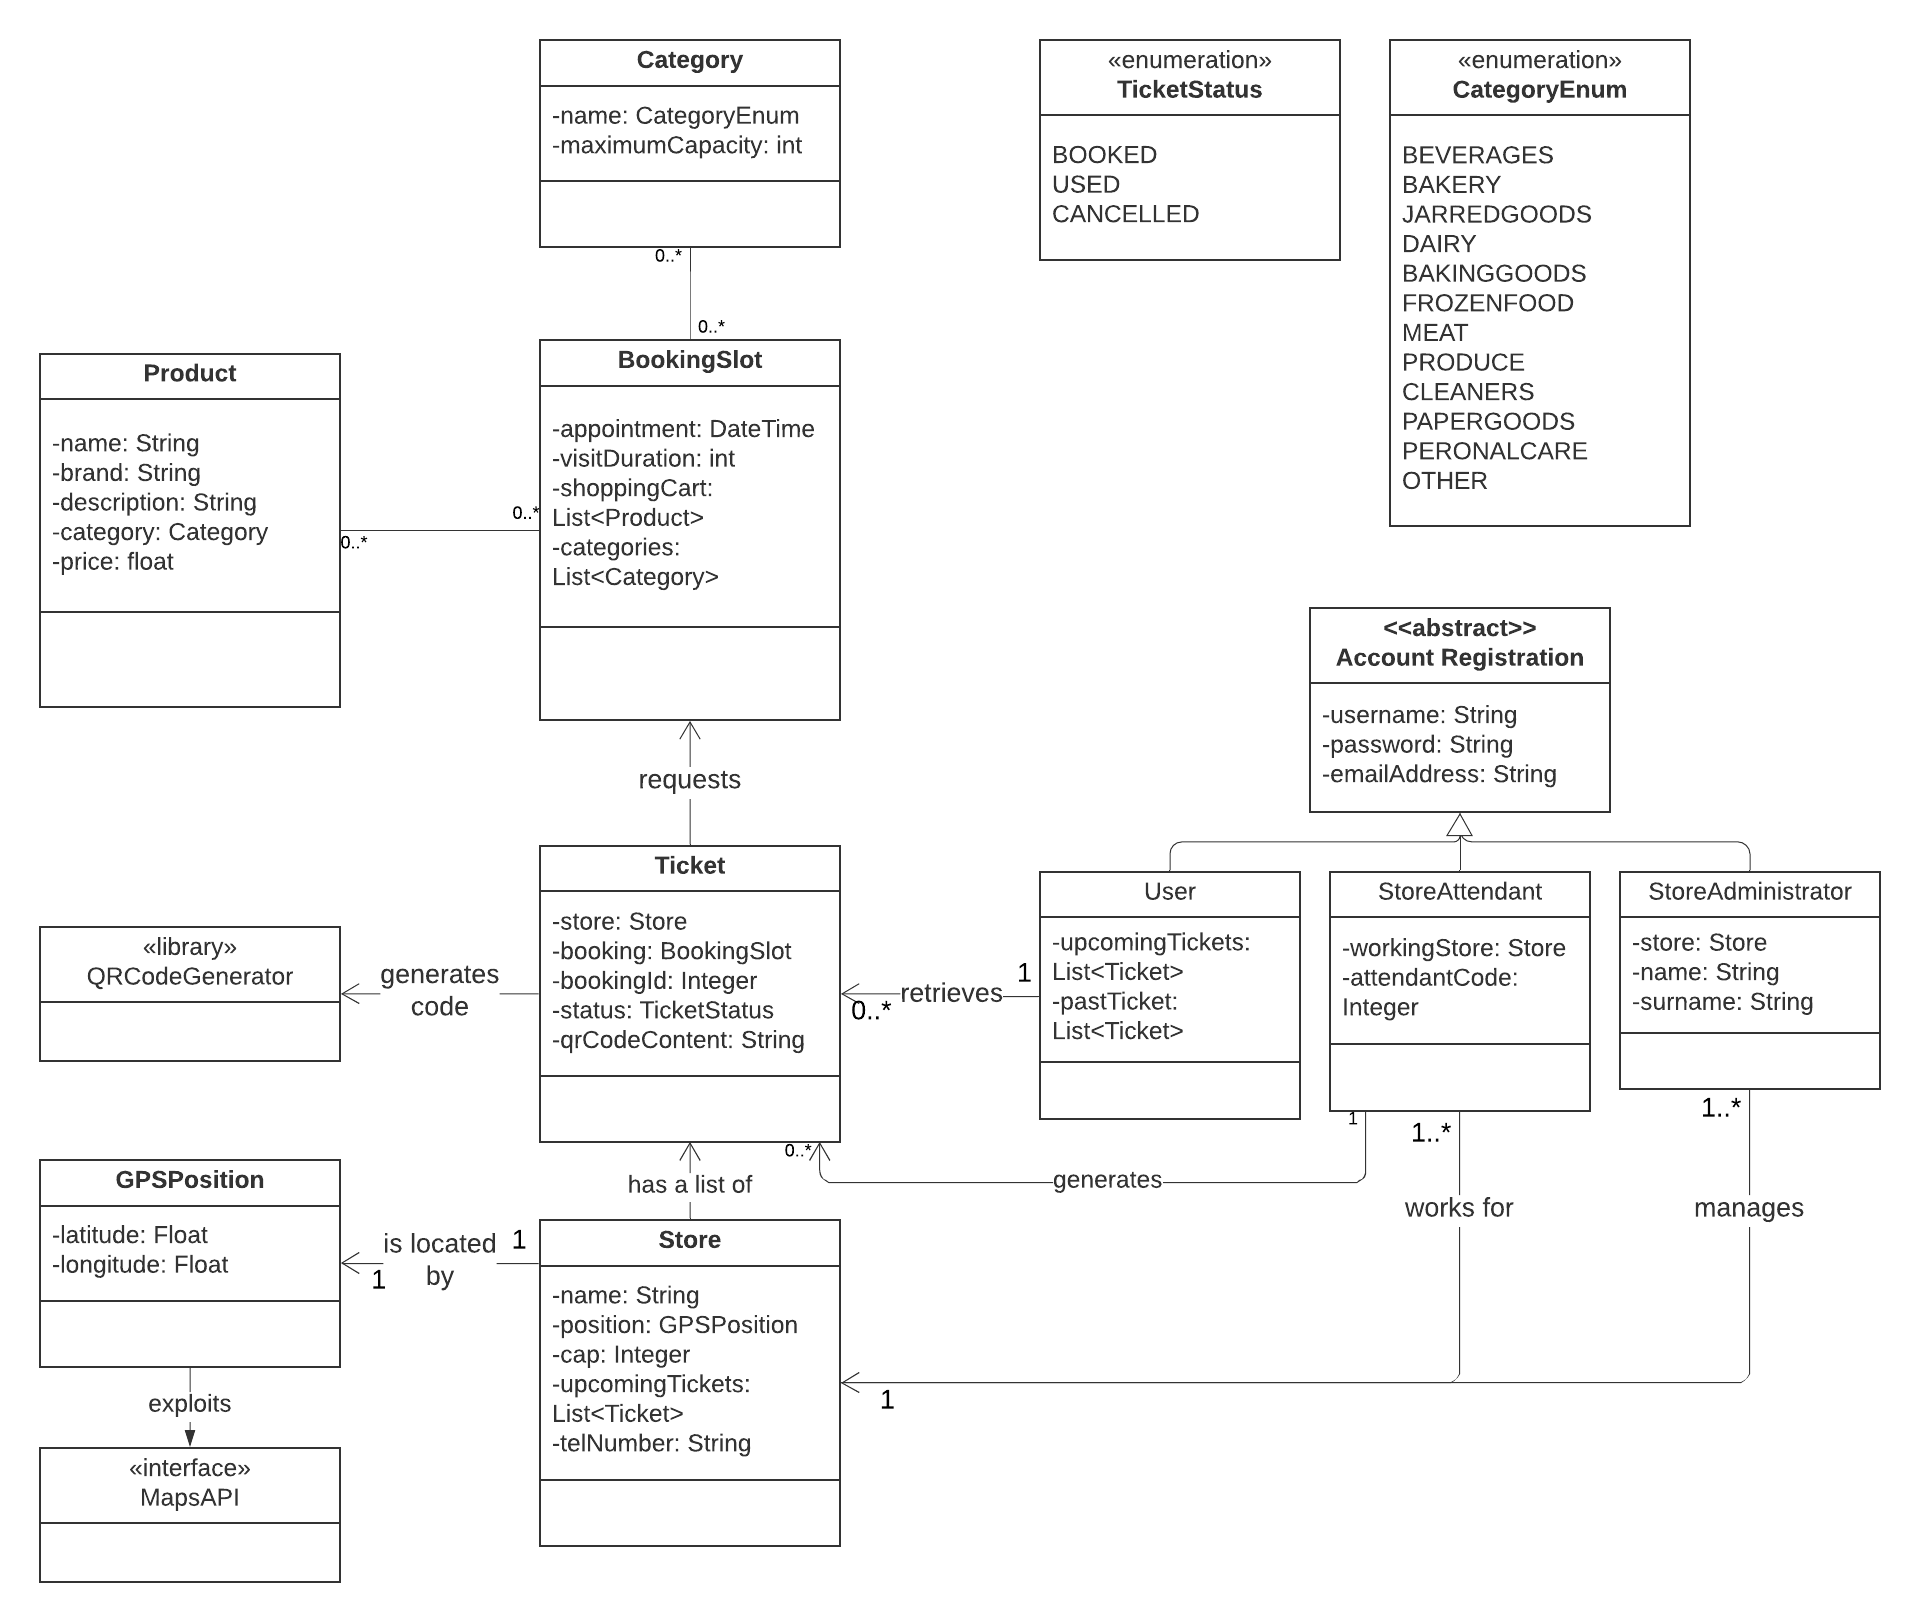
\includegraphics[width=\paperwidth]{assets/UML.png}
        \caption{High-level UML diagram with main classes}
        \label{class_diagram}
    \end{center}

\end{figure}

\subsubsection{User Interfaces}
The system should interface with users through devices which must be connected to the Internet.

Everyone that needs to use this service would connect to it through a Web Interface (from an existent domain, like \textit{www.clup.com}) or through a mobile application that can be installed on smartphones (both IOS and Android).

\subsubsection{Software Interfaces}
CLup will use some important external interfaces in order to accomplish its functionalities.

The first one is a QRCode generator in order to print a check-in code to customers.
The ticket unique ID will be sent to the generator interface, which will return a valid QR representation of it.\\
The code will then be scanned by store attendants for entrances counting.

The second one is an API provided by a map service owner (like \textit{Google Maps} or \textit{OpenStreetMaps}), which will use the position given by the application to return an interactive map with a marker on that exact position.

Another API service used is the one of the DBMS system, which will be adopted in order to query the database in an efficient way.
\subsubsection{Hardware Interfaces}
The system "as it is" does not provide any hardware interface. However, local shops could use the QR Code given by the application on their local systems in order to monitor the number of customers who have entered the shop.
\subsubsection{Hardware Constraints}
Each person interested in using the system described in this document to line up for a shop should have a device connected to the Internet, which could be a smartphone, tablet or personal computer.

The basic requirement is to have an Internet browser installed on the used device.
There is then the possibility of downloading and installing the official CLup application from the most important stores, like Apple's \textit{App Store} or Android's \textit{Play Store}.

Shops, instead, should have some devices connected to the service (through web interface or application) in order to monitor queue length, entrances, generate ticket on the spot and, if needed, anticipately close the booking sessions.

\newpage
\subsection{Product Functions}
\label{product_functions}

<<<<<<< HEAD
\subsubsection{ASAP: As Soon As Possible}

This functionality is accessible to all \textbf{Users} (\ref{User}). The user clicks a button and the system tries to generate the first available ticket for the current day's queue; if the generation fails the system suggests them to book a future visit.
=======
\subsubsection{Line-up}
\label{line_up}
This functionality is accessible to all \textbf{Users} (\ref{User}). The application provides all available slots during the current day and, if the user chooses an unavailable slot, the system suggests them to book a future visit instead.
>>>>>>> a5f1692bbf35015c73cb181eb7af0cbc24bb97fa
Alternatively, the ticket is generated alongside a QR code identifying uniquely users and their queue number. The waiting time is shown to the user until it reaches the last 10 minutes marker alerting them to approach the store.
\begin{figure}[!htb]
    \begin{center}
        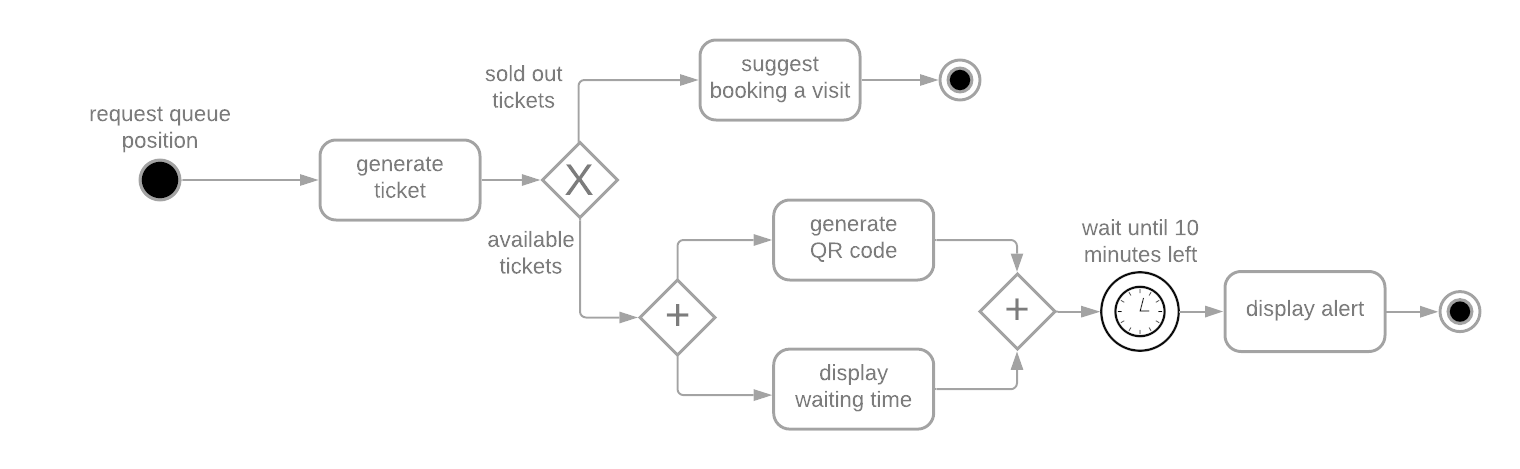
\includegraphics[scale=0.29]{assets/function-line-up.png}
        \caption{BPMN diagram line-up method}
    \end{center}
\end{figure}

\subsubsection{Make a reservation}
\label{book_a_visit}
This functionality is available to every \textbf{User} (\ref{User}). The user accesses the booking through the menu and teh application displays a calendar with all available slots. Alongside this the system suggests               requests a new booking, the system displays all available slots. The service identifies as available a slot with the following requisites: it must be within the capacity allowed by the shop and must include a limited number of customers in order to balance the daily flow to the facility. If the slot is available the user is taken to the last step discussed later on, otherwise the application suggests different results based on the user's choice. They can filter results with the same time of the previous one and be suggested with alternative stores of the same chain or different one; if the user decides otherwise, the system displays alternative days/time slots analyzed from the customer's previous data.
The last step is the optional filling of an hypothetical shopping list and the final confirmation.
\begin{figure}[!htb]
    \begin{center}
        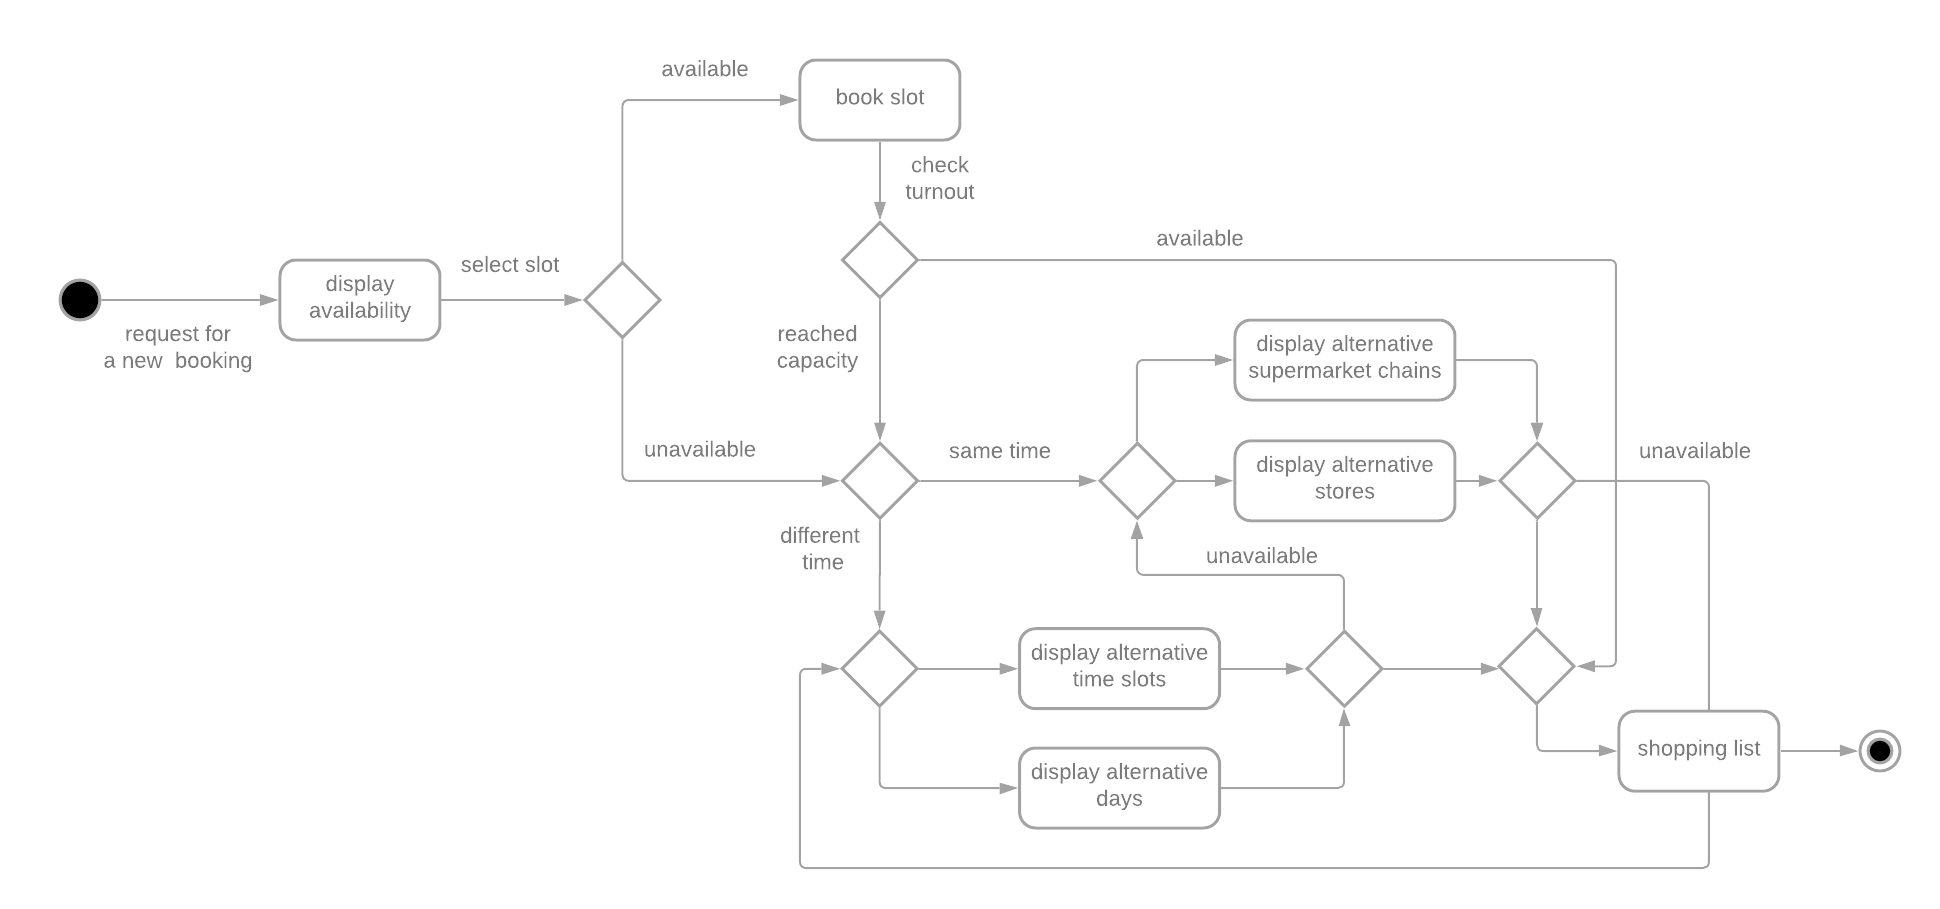
\includegraphics[scale=0.2]{assets/function-book-a-visit.png}
        \caption{BPMN diagram booking method}
    \end{center}
\end{figure}

\subsubsection{Hand out tickets on spot}

This functionality is reserved only for staff members. The customer reaches the supermarket/grocery shop and asks the staff to be queued up. The personnel accesses the system which interacts with the database and generates a ticket, granting the customer a spot in the queue.
\begin{figure}[!htb]
    \begin{center}
        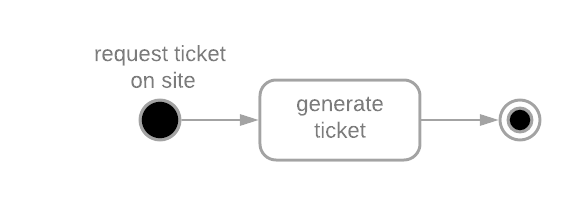
\includegraphics[scale=0.5]{assets/function-hand-up.png}
        \caption{BPMN diagram site method}
    \end{center}
\end{figure}

\subsection{Actors}
\subsubsection{User}
It's a customer, i.e. a normal person who intend to go to the grocery shop. It is able to use the smartphone application or surf on its website. It uses the service in order to access the stores, according to the regulations. It takes advantage in using the application since, when it want to access a store, it retrieves the unique number and can wait from a close and safe building.

\subsubsection{Attendant}
It's a worker of a specific store. Its job is to help customers and monitor the entrances of people. It uses the application for scanning the QR code of users at the entrance of the store. In addition, it can enter in a dedicated section of the application in order to act as an intermediate for those customers who don't have an Internet access.

\subsubsection{Store Administrator}
It's the administrator of a shop or a chain of stores. For the application's purpose only, we identify stores as grocery shops. The store administrator is the person who chooses to adopt the service in order to manage the flows of people inside and outside the building, as well as observing the laws on social distancing.

\subsection{Assumptions, Dependencies, Constraints}
\subsubsection{Assumptions}
\begin{enumerate}[label=\textbf{D\arabic*}:]
    \item GPS position of the shop is exact and leads to that shop.
    \item In case of QR Code entrances monitoring, shop should have an internal system in order to count them.
    \item Each user wanting to use the online service is needed to have a device connected to Internet (such as PC, Mac, smartphone, etc).
    \item There are no connection issues when actors interface with the system.
    \item Each attendant knows the personal code and register to the correct shop.
\end{enumerate}

\newpage
\section{Specific Requirements}
\subsection{Interface Requirements}
\subsubsection{Customer interfaces}
In figure \ref{mock_sign_in_up} we can see the initial screen of the application.
It asks the user to log in or create an account.

In case he decides to create an account, there are three possibilities of subscription (customer, administrator or attendant).\\
In each case, further custom information needs to be provided.

For example, in the case of a Store Administrators, the system would ask them the details of their store (name, position, etc).\\
Instead, in the case of Store Attendants, it would ask them the store in which they are actual working, and their personal attendant code.
\begin{figure}[H]
    \begin{center}
        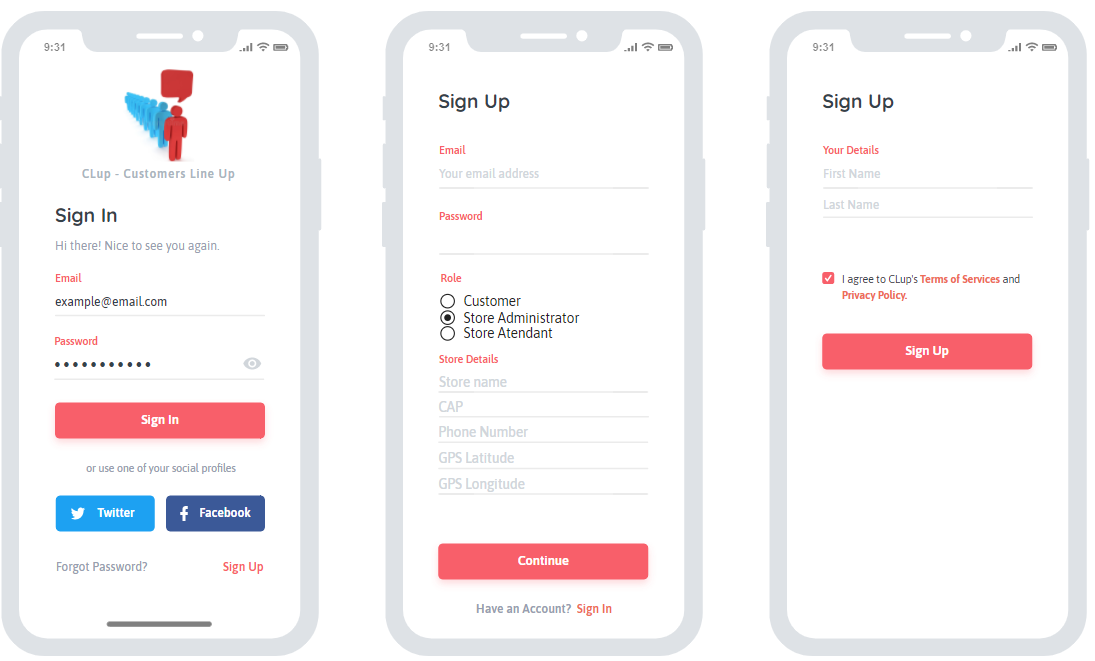
\includegraphics[width=\textwidth]{assets/mock_sign_in_sign_up.png}
        \caption{Sign In and Sign Up procedures.}
        \label{mock_sign_in_up}
    \end{center}
\end{figure}

You can access to bookings page described in figure \ref{mock_bookings} through the contextual menù on the left side of application.\\
Once here, there is the possibility of managing the upcoming bookings or check for the details of them and also for past bookings, which are listed immediately below.

When you are on a details page, all the information about the selected booking is listed. Through a button, it is possible to cancel that booking (if it is an upcoming one).

\begin{figure}[H]
    \begin{center}
        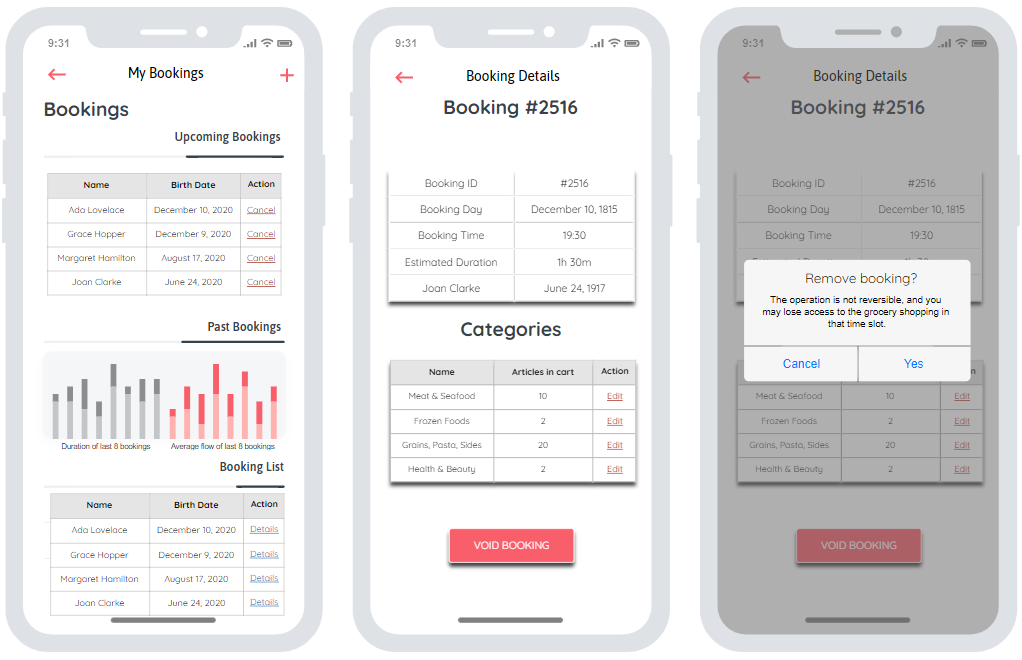
\includegraphics[width=\textwidth]{assets/mock_bookings.png}
        \caption{Home page of the application.}
        \label{mock_bookings}
    \end{center}
\end{figure}

Finally, in figure \ref{mock_new_booking}, you can create a request a new queue number through a dedicated page, as explained in \ref{line_up}.
Otherwise, if you use "Book a visit" function, and the time slot you selected is not available, the system will suggest you another one, as shown in Figure \ref{mock_new_booking_unavailable}.

\begin{figure}[H]
    \begin{center}
        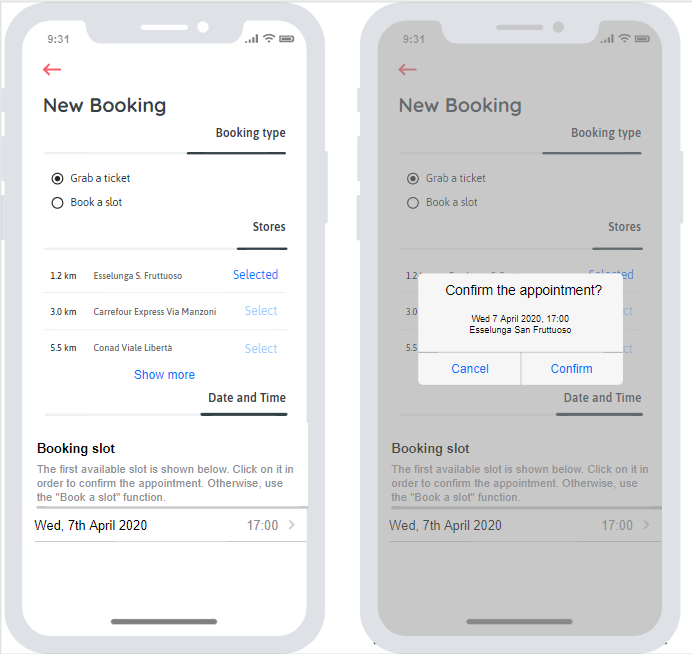
\includegraphics[width=225pt]{assets/mock_line_up.png}
        \caption{Line-up functionality.}
        \label{mock_new_booking}
    \end{center}
\end{figure}

\begin{figure}[H]
    \begin{center}
        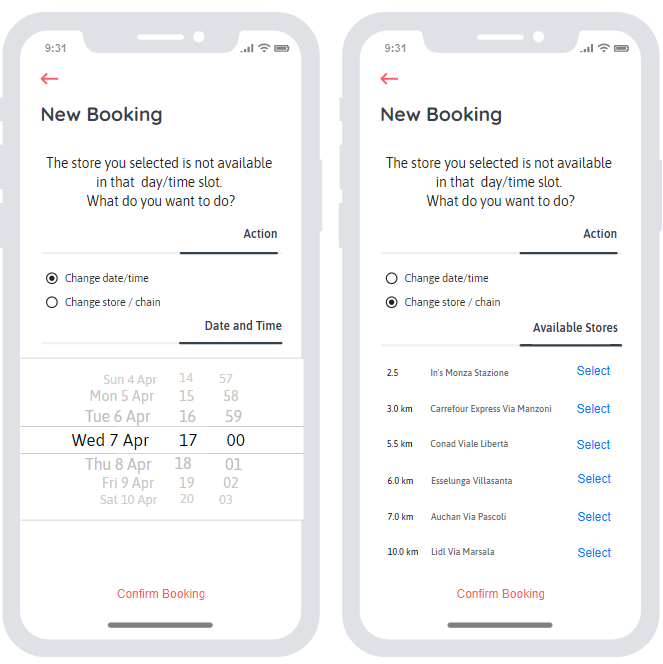
\includegraphics[width=225pt]{assets/mock_new_booking_unavailable.png}
        \caption{"Book a visit" procedure with unavailable date/time.}
        \label{mock_new_booking_unavailable}
    \end{center}
\end{figure}

\subsubsection{Store Administrator interfaces}
In figure \ref{mock_store_admin_home} there is a brief overview of the web interface of Store Administrator.
As it can be seen, there are four macro areas, each one with its own features.
The store administrator can edit information about its grocery shop, its time slot, can manage the attendants and can also see the list of upcoming booking for the shop.
\begin{figure}[H]
    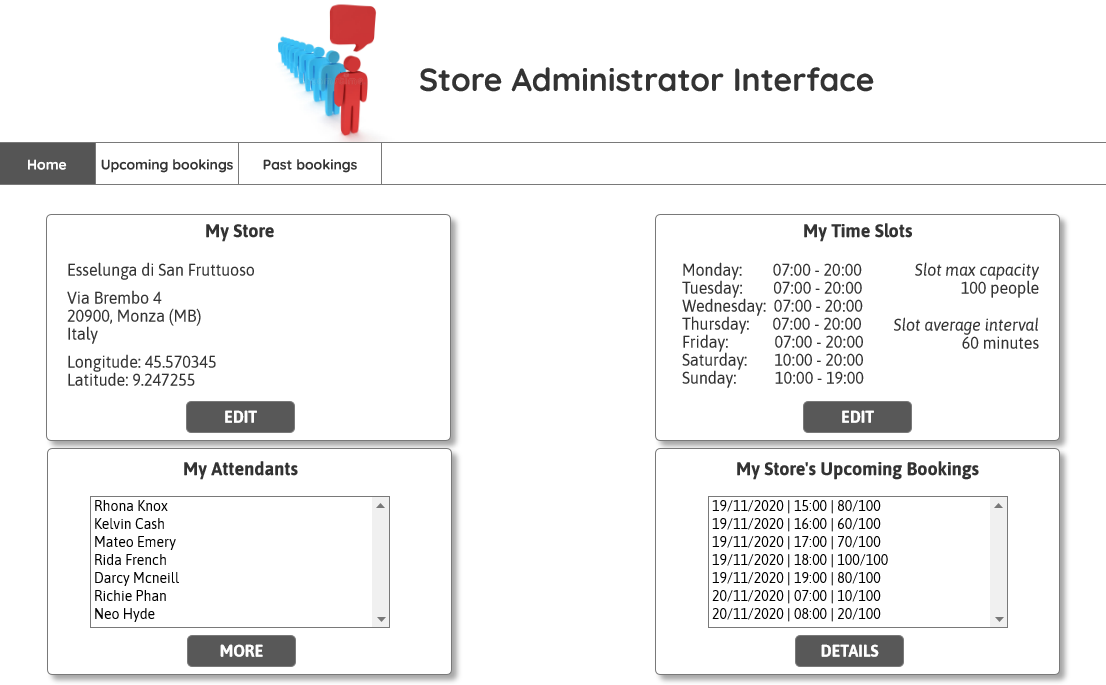
\includegraphics[width=\textwidth]{assets/mock_home_store_admin.png}
    \caption{Store administrator home page}
    \label{mock_store_admin_home}
\end{figure}

\subsubsection{Hardware Interfaces}
As said before, the application "as it is" does not provide any hardware interface.
However, there is the possibility of integration with shops' system and hardware in order to monitor entrances through the given QR code.
\subsubsection{Software Interfaces}
The software, through appropriate APIs, could manage the reading of the QR codes in order to check their validity and their consistence with actual date and time.

\subsection{Functional Requirements}
\subsubsection{User Scenarios}
\textbf{Scenario 1}\\
Alice is an housewife. She lives with her husband and four children in a small village, not too far from Milan. Due to the Covid-19 spread, the government of the region decided to impose a maximum of 30 people inside grocery stores simultaneously. Some days before, Alice went to the nearest supermarket and she discovered there was a queue with more than 50 people in-line; it would take more than two hours for entering, so Alice decided to give up. Just yesterday, the same supermarket launched CLup, an application which helps to manage queues remotely. Alice downloaded it on her smartphone as soon as she discovered it: thanks to CLup she can now retrieve a virtual number and wait for her turn from home, without losing time in a real queue outside the supermarket.\\

\textbf{Scenario 2}\\
Rodolfo is a middle-aged man who lives in Rome. He has CLup installed on his iPhone since the beginning of the lock-down in Italy. Whenever Rodolfo decides it's time to go shopping for some food, he launches the application, he logs in, and he retrieves his number: 355. Rodolfo knows that the nearest Esselunga is the most popular, so it always takes at least 40 minutes until his number is called. For this reason, he starts to watch the latest episode of his favorite tv series. After 30 minutes, the iPhone vibrates: the application CLup is notifying that in 10 minutes the number 355 will be called. Hence, Rodolfo reaches safely the store (there are just a bunch of people who are entering): he shows to the attendant the QR code on the iPhone and he calmly goes to buy the necessary. \\

\textbf{Scenario 3}\\
A full-time student at Politecnico di Milano decided to stay in his apartment in Milan, although he started to follow all the lectures remotely. He studies a lot and he can't go to the grocery store whenever he wants, due to the huge amounts of lessons. But, he uses to go on CLup website and book a slot a couple of days before: he logs in and he goes to the booking section. He selects the date and the time he preferred and one of the nearest available stores. Usually, the system doesn't suggest him other combinations (in order to balance people throughout the day) since he usually books for late evening slots, which are very little frequented. He doesn't even have to insert the expected duration time for the visit since he always stays 30 minutes, so the system autocomplete the field with that value. Then, he selects the list of item's categories he intends to buy: pasta, snacks, beverages, fruits and cleaning. At the end, he confirms everything, and the page displays the QR-code. He clicks on the sharing button and sends it to his smartphone, via Telegram. Once he receives the message, he knows everything worked fine.\\

\newpage
\textbf{Use cases tables}\\

\begin{longtable}{ | c | p{10cm} | }
    \caption{Sign Up User}                                                                                                                                                                                                                                                                    \\

    \hline
                     & Sign Up User on the application                                                                                                                                                                                                                                        \\
    \hline
    Actor            & User                                                                                                                                                                                                                                                                   \\
    \hline
    Entry conditions &
    \begin{itemize}
        \item User has downloaded and opened the application on his smartphone
    \end{itemize}                                                                                                                                                                                                                                                                \\
    \hline
    Events flow      & \begin{itemize}[nosep,after=\strut]
        \item The application displays the Login screen
        \item User clicks on Sign Up button
        \item The application displays a selection list about which account the user intends to create (Customer, Store Administrator or Store Attendant)
        \item User selects the option "Customer" and confirm
        \item The application displays a list of fields that User must compile: Name, Surname, e-mail, municipality, User name, password, date of birth. Some fields are optional: phone number, address, ID of the store card.
        \item User inserts the mandatory data and eventually one or more optional data
        \item User clicks on confirm button
        \item The application displays the acceptance of registration and invite User to go on his inbox in order to confirm the registration
        \item User opens his inbox, checks the e-mails and clicks on confirmation link
    \end{itemize}                                                                                                                                                                                                                                             \\
    \hline
    Exit conditions  & User registration has been successful: user data are stored in the database of the system. User can now Login with his credentials.                                                                                                                                    \\
    \hline
    \hline
    Exception 1      & User insert an e-mail which is already stored in the database. So, after the user inserts his data and clicks on confirm, the application displays an error page which tells that user is already registered to the service and invites him to login with that e-mail. \\
    \hline
    Exception 2      & User inserts an invalid e-mail. So, after user clicks on confirm button, the application displays the same page and an error message, which suggests to the user to check the e-mail inserted or to change it.                                                         \\
    \hline
\end{longtable}

\begin{longtable}{|c| p{10cm}|}
    \caption{Login User}                                                                                                                                                                             \\
    \hline
                     & Login User on the application                                                                                                                                                 \\
    \hline
    Actor            & User                                                                                                                                                                          \\
    \hline
    Entry conditions & \begin{itemize}[nosep,after=\strut]
        \item User has downloaded and opened the application on his smartphone
        \item User has registered to the service
    \end{itemize}                                                                                                                                                    \\
    \hline
    Events flow      & \begin{itemize}[nosep,after=\strut]
        \item The system displays the Login page
        \item User inserts in apposite fields the credentials for logging in and presses the Login button
        \item The system checks the correctness of the credential inserted
        \item The system displays the home page of the application
    \end{itemize}                                                                                                                                                    \\
    \hline
    Exit condition   & User is logged in                                                                                                                                                             \\
    \hline
    \hline
    Exception 1      & User inserts wrong combination of credentials and presses Login button. In this case, the system detects the error and the application displays the Login page with an error. \\
    \hline
\end{longtable}


\begin{longtable}{|c| p{10cm}|}
    \caption{Retrieve a ticket}                                                                                                                                                                                                 \\
    \hline
                     & Retrieve a ticket                                                                                                                                                                                        \\
    \hline
    Actor            & User                                                                                                                                                                                                     \\
    \hline
    Entry conditions & \begin{itemize}
        \item User has logged in
    \end{itemize}                                                                                                                                                                               \\
    \hline
    Events flow      & \begin{itemize}[nosep,after=\strut]
        \item User presses the New Booking button
        \item The application displays two alternatives of booking
        \item User selects the alternative "Retrieve a ticket"
        \item The application displays a confirm page, with the store selected and the time and date of the first slot available
        \item User presses on confirm button
    \end{itemize}                                                                                                                                                                               \\
    \hline
    Exit condition   &
    The application displays the unique ID number of the ticket and the QR-code associated to it                                                                                                                                \\
    \hline
    \hline
    Exception 1      & User presses on confirm button but it has got a ticket in his current bookings, which is still valid. In this case, the application displays an error page which suggests to go on the tickets' section. \\
    \hline
    Exception 2      & User doesn't like the date/time of the first slot available. In this case, it has to press on Cancel button in order to go back to the home page or, in alternative, it can close the application.       \\
    \hline
\end{longtable}



\begin{longtable}{|c| p{10cm}|}
    \caption{Book a visit}                                                                                                                                          \\
    \hline
                     & Book a visit                                                                                                                                 \\
    \hline
    Actor            & User                                                                                                                                         \\
    \hline
    Entry conditions & \begin{itemize}
        \item User has logged in
    \end{itemize}                                                                                                                   \\
    \hline
    Events flow      & \begin{itemize}[nosep,after=\strut]
        \item User presses the New Booking button
        \item The application displays two alternatives of booking
        \item User selects the alternative "Book a slot"
        \item The application displays a page with the day/time slots already available for a certain range (e.g. for the current month or for the next month) for a certain store
        \item User selects the store and the slot he prefers (from the available ones) and clicks on the confirm button
        \item The system estimates the expected duration of the visit based on the analysis of previous visits or, in alternative, it takes a default value
        \item The application displays the visit duration time and a checklist with the categories of products that the customer wants to buy
        \item User selects all the categories he intends to buy (optional) and, eventually, he changes the expected duration time. Then, User clicks on confirm button
        \item The system checks whether if there are better alternatives based on the categories' selections of User
        \item The application displays a page with the summary of all the previous selections and eventually displays other available slots that can balance better with the choices of other customers' reservations
        \item User checks his selections and presses the confirm button
        \item The system adds the booking to the database and generates the unique ID number and the QR code
    \end{itemize}                                                                                                                   \\
    \hline
    Exit condition   & The application displays the summary page of the booking, with the preferences selected by the user, the ID number and the QR code generated
    \\
    \hline
    \hline
    Exception 1      & User has another reservation in the same day. In this case, the application displays an error message and redirect User to the home page.    \\
    \hline
\end{longtable}


\begin{longtable}{|c| p{10cm}|}
    \caption{Remove a booking}                                                                                                                                                                                   \\
    \hline
                     & Remove a booking                                                                                                                                                                          \\
    \hline
    Actor            & User                                                                                                                                                                                      \\
    \hline
    Entry conditions & \begin{itemize}
        \item User has logged in
    \end{itemize}                                                                                                                                                                \\
    \hline
    Events flow      & \begin{itemize}[nosep,after=\strut]
        \item User clicks on a reservation already done
        \item The application answers with the details of the booking selected, such as: booking ID, day and time of the booking, store selected.
        \item User presses the button "Remove"
        \item The application displays a popup with the notice that the booking is going to be removed permanently
        \item User confirms the removal
        \item The system proceeds with the deletion of the booking from the database
    \end{itemize}                                                                                                                                                                \\
    \hline
    Exit condition   & The application notifies that the booking has been removed correctly and it returns to the home page.
    \\
    \hline
    \hline
    Exception 1      & User wrongly presses the delete button. In this case, the application displays the popup with the notice that the booking is going to be removed and the user presses on "Cancel" button. \\
    \hline
\end{longtable}

\subsubsection{Attendant Scenarios}
\textbf{Scenario 4}\\
Hassan works at the new Coop located in Marsala street in Monza. Once the store decided to adopt CLup for the management of flows in and out the supermarket, the manager of Hassan assigned him the task of monitoring the main entrance. Therefore, Hassan downloaded the application and registered as a staff member. Hassan's job is to scan the QR code of the customers with his smartphone, and to make sure that everything works fine. The application always displays a counter, so that Hassan can know exactly how many people there are inside the store. However, it does never happen that the counter reaches the maximum value allowed for laws. Hassan is happy for the introduction of CLup because it has got everything needed so that his job became very easy.\\

\textbf{Scenario 5}\\
Salvatore is a young boy who lives in a little village near Marsala, in Sicily. The chain of supermarkets where he works as an assistant has introduced a new application for managing queues, in order to avoid gatherings outside its buildings. However, Salvatore knows that there are a lot of elderly people in his village, so how can they use the application without even having a smartphone? Surprisingly, Salvatore came to know that the service has got a function which allows him to act as an intermediate for the aged people who come to his store. His job now is to log in on the application as a staff member and take the credentials of customers who need help. After that, he asks to customers when they want to come again, so that he can reserve them a slot. The application generates the QR code, which he prints and gives to the customer. Salvatore's days are full of work now, because there are a lot of old ladies who need an help, but he knows he must done his job for community's sake.\\

\textbf{Attendant use case tables}\\

\begin{longtable}{|c| p{10cm}|}
    \caption{Scan QR code}                                                                                                                                                                                                                                                                \\
    \hline
                     & Scan QR code                                                                                                                                                                                                                                                       \\
    \hline
    Actor            & Store Attendant                                                                                                                                                                                                                                                    \\
    \hline
    Entry conditions & \begin{itemize}
        \item Store Attendant has logged in
    \end{itemize}                                                                                                                                                                                                                                         \\
    \hline
    Events flow      & \begin{itemize}[nosep,after=\strut]
        \item Store Attendant presses on the button "Scan"
        \item The application displays a page with the QR code scanner
        \item The attendant frames a QR code
        \item The system reads the QR code and checks if it is associated to an acceptable reservation, according to the actual date, time and location
        \item The application notifies whether if the QR code is valid
    \end{itemize}                                                                                                                                                                                                                                         \\
    \hline
    Exit condition   & The application displays a page with the total number of people inside the store at that moment
    \\
    \hline
    \hline
    Exception 1      & The system cannot read the QR code. In this case, the application displays an error status which invites the attendant to frame the QR code again.                                                                                                                 \\
    \hline
    Exception 2      & The system cannot read the QR code for 3 times consecutively. In this case, the application displays an error status which invites the attendant to make sure that the QR code is original.                                                                        \\
    \hline
    Exception 3      & The system reads a QR code with an unacceptable day/time/store reservation. In this case, the application displays the details of the reservation in order to show where is the problem (e.g. it's too early or too much late or it isn't the correct date/store). \\
    \hline
\end{longtable}

\begin{longtable}{|c| p{10cm}|}
    \caption{Release a ticket}                                                                                                                                                      \\
    \hline
                     & Release a ticket                                                                                                                                             \\
    \hline
    Actor            & Store Attendant                                                                                                                                              \\
    \hline
    Entry conditions & \begin{itemize}
        \item Store Attendant has logged in
        \item The application is connected with a working printer
    \end{itemize}                                                                                                                                   \\
    \hline
    Events flow      & \begin{itemize}[nosep,after=\strut]
        \item Store Attendant presses on the button "Release a ticket"
        \item The application displays a page with a list of fields to be filled, such as Customer Name, Customer Surname, Store and it shows the available slots for the current day and for the next days for the store selected
        \item Store Attendant completes all fields with Customer's information and presses on "Confirm" button
        \item The application displays the confirmation page with a summary of the data inserted
        \item The attendant checks the data are correct and confirms
        \item The system inserts the new ticket in the database and generates the unique ID number and the QR code associated
        \item The application displays a page with the QR code
        \item Store Attendant clicks on "print" button
        \item The application generates the pdf to print with all the necessary data of the ticket and sends it to the printer
    \end{itemize}                                                                                                                                   \\
    \hline
    Exit condition   & The application notifies that the pdf is going to be printed and it displays the home page of Store Attendant
    \\
    \hline
    \hline
    Exception 1      & There are not slots compatible with customer's desires. In this case, Store Attendant can cancel the procedure and the application returns to the home page. \\
    \hline
    Exception 2      & The printer returns an error. In this case, the application deletes from the database the ticket generated and displays an error message.                    \\
    \hline
\end{longtable}

\begin{longtable}{|c| p{10cm}|}
    \caption{Delete a reservation}                                                                                                                              \\
    \hline
                     & Delete a reservation                                                                                                                     \\
    \hline
    Actor            & Store Attendant                                                                                                                          \\
    \hline
    Entry conditions & \begin{itemize}
        \item Store Attendant has logged in
    \end{itemize}                                                                                                               \\
    \hline
    Events flow      & \begin{itemize}[nosep,after=\strut]
        \item Store Attendant presses on the button "delete a reservation"
        \item The application displays a page with the list of all the tickets generated by all the Store Assistant of that store and a search bar
        \item Store Attendant clicks on the search bar and inserts the name and surname of a customer
        \item The system checks the record in the list and displays the results
        \item Store Attendant selects the record he wants to delete and presses on "delete" button
        \item The application displays a page with the summary of the reservation selected
        \item Store Attendant clicks on "confirm" button
        \item The system deletes the reservation from the database and displays a message of deletion completed
    \end{itemize}                                                                                                               \\
    \hline
    Exit condition   & The application returns to the home page
    \\
    \hline
    \hline
    Exception 1      & The system doesn't find any record associated to the name and surname inserted. In this case, the application displays an error message. \\
    \hline
\end{longtable}

\subsubsection{Store Administrator Scenarios}
\textbf{Scenario 5}\\
The Esselunga store located in San Fruttuoso (Monza) imposed a maximum limit of 100 people inside the store at the same moment, in order to observe the regulations of government. Due to this, a long queue always forms, from the entrance of the supermarket to the church of Triante's neighborhood. For this reason, Marco, which is the store administrator in action on the territory of Monza and Brianza, decided to adopt CLup in his stores.
Thanks to CLup the customers can now take reservations and waiting their turn from home, avoiding the formation of queues and crowds nearby the stores.\\

\textbf{Scenario 6}
Giannamaria is the manager of the biggest grocery shop in Rome. The store can contain more than a thousand people at the same time, in normal conditions, but due to the coronavirus spread and the consequent laws about social distancing inside buildings, the store must limit the number of entrances at a maximum of 300 people. Giannamaria always thought it would have been difficult to keep track of the people entering and exiting in such a big store, so she immediately decided to adopt CLup. Thanks to the application, she can make use of only a couple of attendants in order to managing the entrances, and she can know exactly how many people there are in the store, at any time, through the Store Administrator section. Moreover, she can easily manage time slots and change timetables with few procedures, through the application. According to Giannamaria, the managing of the store has never been so easy: in fact, she is thinking about to continue to use CLup even after the virus situation has been solved.

\textbf{Scenario 7}
The manager of Eurospin's chain of discount in Italy asked to the store administrators of each area to draw up a document about the more frequented hours of their customers. Months ago, the stores converted to the use of CLup application. Therefore, the store administrators of each area can make use of it in order to write the document and make statistics. In fact, the application has a section, only for the store administrators, where they can see the list of all the upcoming and all the past bookings made in a specific store by the customers, with all the necessary details. So, the store administrators export the list on an Excel file and, starting from that, they can quickly make all the statistics they need to.

\begin{longtable}{|c| p{10cm}|}
    \caption{Modify time slots}                                                                                                                                              \\
    \hline
                     & Modify time slots                                                                                                                                     \\
    \hline
    Actor            & Store Administrator                                                                                                                                   \\
    \hline
    Entry conditions & \begin{itemize}
        \item Store Administrator has logged in
    \end{itemize}                                                                                                                            \\
    \hline
    Events flow      & \begin{itemize}[nosep,after=\strut]
        \item Store Administrator goes to "My Time Slots" section and clicks on the edit button
        \item The system extract the data from the database and the application displays the required information, such as: name of the store, location, capacity of the store, time of the slots, opening hours.
        \item Store Administrator makes his modifications, for example extending the opening hours of the store, and it clicks on confirm button
        \item The application checks whether if the changes are acceptable and then it displays a confirm page with the summary of the changes
        \item Store manager confirms again
    \end{itemize}                                                                                                                            \\
    \hline
    Exit condition   & The application displays a page with the updated information of the store
    \\
    \hline
    \hline
    Exception 1      & Store Administrator inserts unacceptable value of time. In this case, the system detects the inconsistency of the data and displays an error message. \\
    \hline
\end{longtable}

\begin{longtable}{|c| p{10cm}|}
    \caption{View Upcoming Bookings Details}                                                                                                                             \\
    \hline
                     & View Upcoming Bookings Details                                                                                                                    \\
    \hline
    Actor            & Store Administrator                                                                                                                               \\
    \hline
    Entry conditions & \begin{itemize}
        \item Store Administrator has logged in
    \end{itemize}                                                                                                                        \\
    \hline
    Events flow      & \begin{itemize}[nosep,after=\strut]
        \item Store Administrator goes to upcoming bookings section and clicks on the "Details" button
        \item The system takes from the database the list of all the reservations made for that store and the application displays the list
        \item Store Administrator clicks on one of the bookings
    \end{itemize}                                                                                                                        \\
    \hline
    Exit condition   & The application displays a page with the details of the selected booking, such as: ID of the ticket, date and time, list of product's categories.
    \\
    \hline
    \hline
    Exception 1      & CLup application cannot reach the database. In this case, an error message is displayed.                                                          \\
    \hline
\end{longtable}


\todo . Tables: lista dei clienti, generatore statistiche prenotazioni, modifica dati o time slots

\subsubsection{Requirements}
This subsection summarizes the goals describe in \ref{goals}, showing the requirements and the domain assumptions for each of them.

\begin{enumerate}[label=\textbf{G\arabic*}:]
    \item {Allow users to retrieve a unique queue number
          \begin{itemize}
              \item
          \end{itemize}
          }
    \item {Allow users to generate a QR Code
          \begin{itemize}
              \item
          \end{itemize}
          }
    \item {Allow shops to offer CLup service
          \begin{itemize}
              \item
          \end{itemize}
          }
    \item {Allow users to "book a visit"
          \begin{itemize}
              \item
          \end{itemize}
          }
    \item {Let the system to infer a visit duration
          \begin{itemize}
              \item
          \end{itemize}
          }
    \item {Allow users to receive a suggestion of alternative slots
          \begin{itemize}
              \item
          \end{itemize}
          }
    \item {Allow users to receive notifications on available slots
          \begin{itemize}
              \item
          \end{itemize}
          }
\end{enumerate}

\subsubsection{Traceability Matrix}
\begin{table}[H]
    \begin{center}
        \begin{tabular}{|l|l|}
            \hline
            \textbf{Requirement} & \textbf{Use case} \\
            \hline
        \end{tabular}
        \caption{Traceability matrix schema.}
    \end{center}
\end{table}

\subsection{Performance Requirements}
Of course, the system should have a good response time, which could be included between 0.1 and 2 seconds.
Otherwise, customers and store workers may think that the service is interrupted or does not work.

The average workload of the system is expected to be very high, because of its principal functionality. However, it depends on the number of stores that would adopt it.
With a rough calculation, the system must guarantee at least 1 billion of operations per day.

Through a good distribution of the application it is possible to accomplish this specific requirement.

\subsection{Design constraints}
\subsubsection{Hardware Constraints}
On stores side, each attendant is required to have a device from which it is possible to check-in customers by scanning their QR Code.
For this functionality stores could have a Barcode Reader connected through usb to a personal computer or, otherwise, they could use a mobile application connected to their system.

Each customer, instead, must have a mobile device on which grab a ticket or make a reservation.

\subsubsection{Privacy Constraint}
The system, since the main application area is the european one, must be compliant to EU's GDPR law. Furthermore, the data must pass through a secure connection, in order to prevent \textit{Man in the Middle} attacks.

When a customer, store attendant or store manager registers to the application, the privacy policy must be read and accepter. Otherwise, the user will not be able to use the service.

\subsection{Software System Attributes}
\subsubsection{Easy usability}
The system must be very easy to use, because the user base target is various.

In fact, anyone needs to go to grocery shop, from the teenager to the elderly man or woman.

The application should then be accessible to anyone in this age range. Of course, in case of people who can not use this system, there is the possibility of manual grabbing ticket on the spot.
\subsubsection{Reliability}
The system must prevent downtime, in order to let people going to the grocery shop in the opening hours. \\
The highest number of simultaneous accesses is expected in the most frequented shopping hours (early morning or late afternoon).
\subsubsection{Availability}
The system must be available as much as possible, with a minimum value of 96\% of time.
\subsubsection{Security}
Communication between parties are encrypted and goes on a secure channel (through SSL protocol).

Furthermore, the database guarantees that performed operations are always authorized (\textit{e.g.. a customer cannot modify information of a store}).
\subsubsection{Cross Platform}
The system must be supported on the principal operating systems, either mobile and computers. It is in any case usable on every web browser, from every device.

The downloadable application, instead, must be supported by Windows, Linux, Mac OS, IOS and Android.
\subsubsection{Maintainability}
The system must be designed in such a way that permits future addition of functionalities with minimum effort.
Design techniques must in fact guarantee an high reusability.
\newpage
\section{Formal Analysis}
\newpage
\section{Effort spent}
\begin{tabular}{ | l || c | c | c | c |}
    \hline
    Student        & Time for S.1 & Time for S.2 & Time for S.3 & Time for S.4 \\ \hline
    Alice Piemonti & 3h           & 20 min       & 9h           &              \\ \hline
    Luca Pirovano  & 3h           & 6h           & 8h           & 3h           \\ \hline
    Nicolò Sonnino &              &              &              &              \\
    \hline
\end{tabular}
\end{document}